\documentclass[a4paper,12pt]{article}

% Packages
\usepackage{float}
\usepackage[utf8]{inputenc}
\usepackage{fancyhdr}
\usepackage[left = 0.6 in, right = 0.6 in, top = 1 in, bottom = 1 in, headsep = 0.5 in]{geometry}
\usepackage[normalem]{ulem}
\usepackage{enumerate}
\usepackage{pgfplots}
\usepackage{titling}
\pgfplotsset{width=8cm,compat=1.9}
\usepackage{stackengine}
\usepackage{algorithm}
\usepackage[noend]{algpseudocode}
%\pagenumbering{gobble} 
\usepackage{amsmath} % add [fleqn] before {amsmath} to left center
\usepackage{amssymb}
\usepackage[T1]{fontenc}
\usepackage{fancybox}
\usepackage{longtable}


\hfuzz = 100pt

%%% Horizontal Line Command
\makeatletter
  \newcommand*\variableheghtrulefill[1][.4\p@]{%
    \leavevmode
    \leaders \hrule \@height #1\relax \hfill
    \null
  }
\makeatother
%%%

%%% Algorithm commands
\algblock{Input}{EndInput}
\algnotext{EndInput}
\algblock{Output}{EndOutput}
\algnotext{EndOutput}
\newcommand{\Desc}[2]{\State \makebox[3em][l]{#1}#2}
%%%

%%% Base conversions
% expandable loop (used to avoid scope problems in tabular cells with the
% standard \loop)
\def\boucle #1\repeat {#1\b@@cle {#1}\repeat \repeat }
\def\b@@cle #1{\repeat #1\b@@cle {#1}}

\makeatletter
\newcount\@nn
\newcount\@mm
\newcount\@base
\newcount\@baseminusone

% please do not use this at home
% #1 must be a counter name, not something expanding to a number.
\def\@arabalpha #1{\ifcase #10\or1\or2\or3\or4\or5\or6\or7\or8\or9\or 
A\or B\or C\or D\or E\or F\or G\or H\or I\or J\or K\or L\or M\or N\or O\or
P\or Q\or R\or S\or T\or U\or V\or W\or X\or Y\or Z\fi}

\newcommand{\baseexpansion}[2][2]{% no negative numbers please!
\def\@digits{}%
\@base#1\relax \@baseminusone\@base\advance\@baseminusone-1
\@nn #2\relax  % this is the number to be written in base #1
%
\ifnum\@baseminusone<36
\def\onerow{#1\kern.1em\hbox{\vrule
   \vtop {\hbox{\ \the\@nn}\kern.3ex\hrule height.1ex }} &%
   \global\@mm\@nn \global\divide\@mm\@base 
   \multiply\@mm\@base \advance\@nn-\@mm 
   \the\@nn \xdef\@digits{\@arabalpha\@nn\@digits}}%
\else
\def\onerow{#1\kern.1em\hbox{\vrule
   \vtop {\hbox{\ \the\@nn}\kern.3ex\hrule height.1ex }} &%
   \global\@mm\@nn \global\divide\@mm\@base 
   \multiply\@mm\@base \advance\@nn-\@mm 
   \the\@nn \xdef\@digits{\the\@nn.\@digits}}%
\fi
%
\leavevmode\oalign{$#2_{10}:$\hfil\cr
      $\left.
      \begin{tabular}{r|l}
         \boucle \onerow \\ \ifnum\@nn>\@baseminusone\global\@nn\@mm \repeat
      \end{tabular}\right\rbrace=
      \mathtt{\@digits}_{#1}$}}     % \hfil removed from the macro

\makeatother

%%% Logic Circuits
\usetikzlibrary{arrows, shapes.gates.logic.US, calc}
\tikzstyle{branch}=[fill, shape=circle, minimum size=3pt, inner sep=0pt]

%%% Header & Footer
\fancyhf{}
\renewcommand{\footrulewidth}{0.1mm}
\fancyhead[L]{Matteo Esposito}
% \fancyhead[R]{COMP 228-AA}
\fancyfoot[R]{\thepage}
\pagestyle{fancy}

%%% Code formatting
\def\code#1{\texttt{#1}}
\renewcommand\maketitlehooka{\null\mbox{}\vfill}
\renewcommand\maketitlehookd{\vfill\null}
\setlength{\abovedisplayskip}{2pt}
\setlength{\belowdisplayskip}{3pt}

%%% Custom settings
% \setlength{\parskip}{1em}  % Paragraph spacing
\setcounter{section}{-1} % Page numbers to start on page 1
\setlength\parindent{0pt} % Remove indenting from entire file
\def\layersep{2.5cm}

%%% Titlepage
\title{\textbf{ArXiv Article Classification}}
\author{Fundamentals of Machine Learning}
\date{Matteo Esposito (20173298)}

%--------------------------------------------------------------------------%

\begin{document}

\begin{titlingpage}
  \maketitle
  \centering
  \vfill
  {\large{University of Montreal}}\par
  {\large{}}
\end{titlingpage}

\newpage

\section{Introduction}

This report will cover the efforts related to the classification of articles on the popular scientific research paper distribution website, \code{arxiv.org}. 

\medskip

More specifically, given the abstract of several thousand papers, our goal was to classify them into one of the following categories: astro-ph.GA, math.AP, astro-ph.CO, math.CO, stat.ML, cs.LG, gr-qc, astro-ph, astro-ph.SR, hep-th, physics.optics, hep-ph, cond-mat.mtrl-sci, cond-mat.mes-hall, quant-ph.

\section{Feature Design}

Since at the lowest level we were interested in the count of unique words in our training set abstracts, our feature design could be seen as a dataset condensing/cleaning exercise. All efforts to tidy the dataset were done to reduce the number of unique words/strings (grouping of string characters between spaces) down from over 65,000 to 21,253 which speeds up computation times significantly. 

\medskip

\underline{Note:} All cleaning functions were implemented using the following syntax (adapted from the TA's OH notebook): 

\begin{verbatim}
    df[t] = df[t].apply(lambda x : re.sub("<regex pattern>", " ", x))
\end{verbatim}

More specifically, the following changes were done:

\begin{enumerate}
    \item Remove newline characters
    \item Remove punctuation
    \item Remove dollar signs and any mathematical symbols (very important given that many abstracts had mathematical terms and functions)
    \item Remove standalone integers 
    \item Make all strings lowercase
    \item Strip all strings of spaces (using x.strip())
    \item Remove all common stopwords
\end{enumerate}

\section{Algorithms}

The algorithms considered and implemented in this kaggle were the following:
\begin{itemize}
    \item Random Classifier
    \item Bernoulli Naive Bayes Classifier using base python + numpy
    \item Multinomial Naive Bayes Classifier from the sklearn library including the use of CountVectorizer, TfidfTransformer and Pipeline.
    \item Support Vector Machine Classifier from the sklearn library including the use of CountVectorizer, TfidfTransformer and Pipeline.
\end{itemize}

\section{Methodology}



\section{Results}

\begin{figure}[H]
    \centering
    \caption{Random Classifier Accuracy Comparison}
    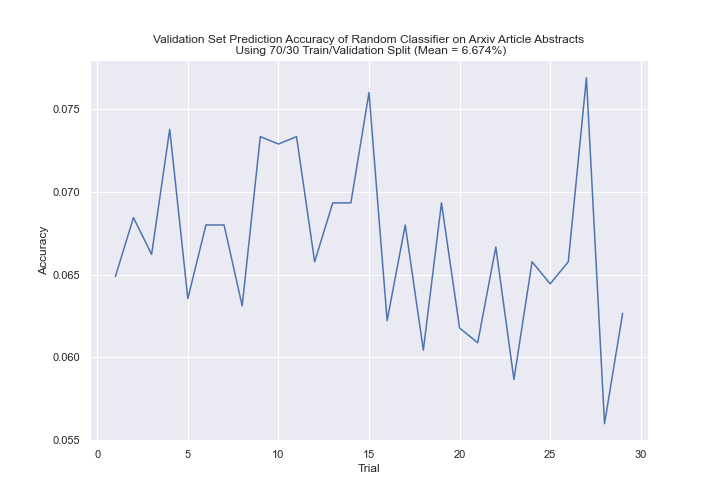
\includegraphics[width=12cm]{compareRandom.png}    
\end{figure}

\begin{figure}[H]
    \centering
    \caption{Bernoulli NB and Multinomial NB Accuracy Comparison}
    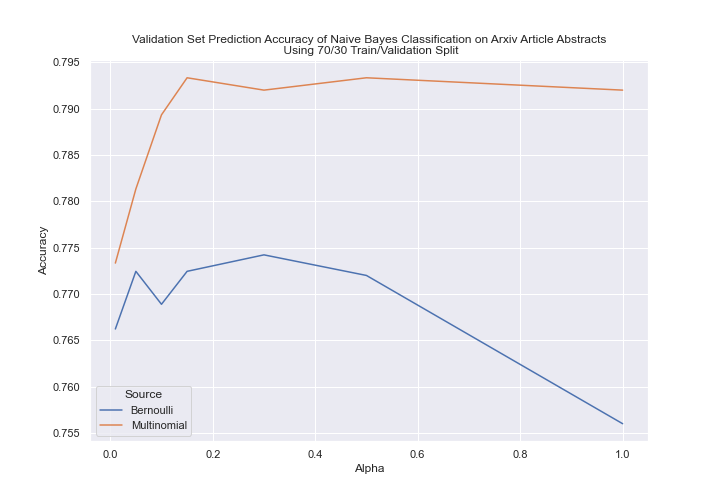
\includegraphics[width=12cm]{compare.png}    
\end{figure}

\begin{figure}[H]
    \centering
    \caption{SVM Grid Search Results}
    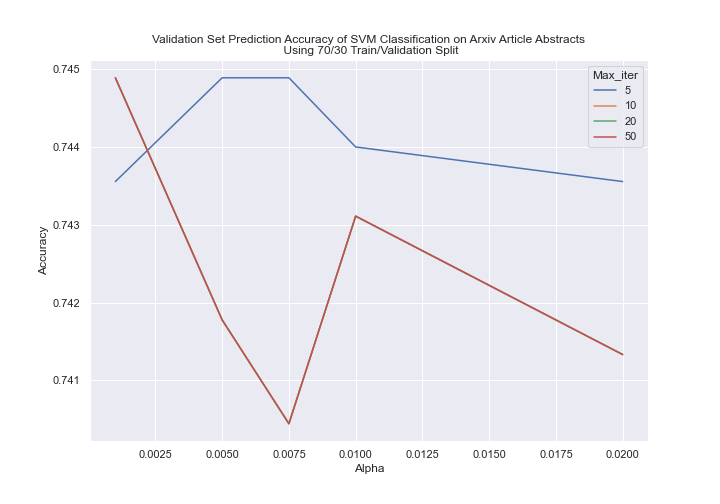
\includegraphics[width=12cm]{compareSVM.png}    
\end{figure}

\section{Discussion}



\section{References}




% \textbf{a)} Since $2^6 = 64$ and $2^7 = 128$, if we are dealing with 87 unique instructions it is clear that we need 7 out of the 24 available bits from the standard word size to represent our instruction/opcode set.

% \textbf{b)} Since we have 17 remaining bits for memory addresses, the maximum value that can be represented in binary is $2^{18}-1 = 262143_{10}$.

% \textbf{c)} Knowing that the range of N-bit 2s complement values is $[-2^{n-1}, 2^{n-1}-1]$, and considering that we have 24 bit words, the range and max of 2s complement values is: 

% $$[-2^{n-1}, 2^{n-1}-1] = [-2^{23}, 2^{23}-1] = [-8388608, 8388607] \Rightarrow \fbox{8388607}$$

% \subsection*{Question 2}

% Interpreting each set of 4 bits from the Marie snippet \code{121830F46000900A}, where bit 1 represents the instruction number and bits 2-4 the memory address, we get the 4 following instructions:

% \begin{table}[H]
%     \centering
%     \begin{tabular}{|c|c|c|c|}
%         \hline
%         \text{\textbf{Hex}} & \text{\textbf{Opcode}} & \text{\textbf{Address}} & \text{\textbf{Instruction}} \\ \hline
%         1218 & 1 = \code{LOAD} & $218_{16}$ & \code{LOAD 218} \\ \hline
%         30F4 & 3 = \code{ADD} & $0F4_{16}$ & \code{ADD 0F4} \\ \hline
%         6000 & 6 = \code{OUTPUT} & - & \code{OUTPUT} \\ \hline
%         900A & 9 = \code{JUMP} & $00A_{16}$ & \code{JUMP 00A} \\ \hline
%     \end{tabular}
% \end{table}

% \subsection*{Question 3}

% % \begin{figure}[H]
% %     \centering
% %     \caption{Timing digram for \code{LOADI} instruction}
% %     \includegraphics[width=12cm]{figures/q3.jpg}    
% % \end{figure}

% \subsection*{Question 4}

% \textbf{a)} Converting every bit in $AAFB1609_{16}$ to binary, we get,

% $$AAFB1609_{16} = 10101010111110110001011000001001_{2}$$

% Converting this to two's complement notation (flip all bits and add 1) we get,

% $$10101010111110110001011000001001_{2} \rightarrow 
% -(01010101000001001110100111110110_{2})$$

% then,

% $$-(01010101000001001110100111110110_{2}) + 1 =
% -(01010101000001001110100111110111_{2})$$

% converting back to decimal,

% $$-(01010101000001001110100111110111_{2}) = -1426385399$$

% \textbf{b)} Converting every bit in $0916FBAA_{16}$ to binary, we get,

% $$0916FBAA_{16} = 00001001000101101111101110101010_{2}$$

% Using the IEEE standard for single precision floating point numbers, namely to use bit 1 as the sign bit, the next 8 for the exponent and remaining 23 for the mantissa we get,

% $$0|00010010|00101101111101110101010$$

% This yields an exponent value of $00010010_2 = 18_{10}$. If we inversely apply the bias to get the original value of the exponent, we have 18 - 127 = -109. If we convert the mantissa, we get $1.00101101111101110101010_{2} \; x \; 2^{-109}$. We will translate the solution by 1 power to the right. $0.1001 0110 1111 1011 1010 1010_{2} \; x \; 2^{-108}$. Converting to hex then decimal we get the following:

% \begin{align*}
%     0.96FBAA_{16} \; x \; 2^{-108} &= (9\cdot16^{-1} + 6\cdot16^{-2} + 15\cdot16^{-3} + 11\cdot16^{-4} + 10\cdot16^{-5} + 10\cdot16^{-6}) \; x \; 2^{-108} \\
%     &= 0.589777589 \; x \; 2^{-108}        
% \end{align*}

% Converting $2^{-108}$ to an exponent of 10, we get:

% \begin{align*}
%     2^{-108} &= 10^{x} \\
%     -108 \cdot log_2(2) &= x\cdot log_2(10) \\
%     \frac{-108}{log_2(10)} &= x \\
%     -32.5112395 &\approx x
% \end{align*}

% finally,

% $$0.589777589 \; x \; 2^{-108} = 0.589777589 \; x \; 10^{-32.5112395}$$

% To get a whole number exponent, we can multiply the coefficient by a constant.

% $$\frac{0.589777589}{10^{-33+32.5112395}} \; x \; (10^{-32.5112395})*(10^{-33+32.5112395}) = 1.8173926 \; x \; 10^{-33}$$

% \subsection*{Question 5}

% $$Q = (A+B)/C - D*E$$

% \textbf{a)} 

% \begin{align*}
%     &\code{Push A} \\
%     &\code{Push B} \\
%     &\code{add} \\
%     &\code{Push C} \\
%     &\code{Div} \\
%     &\code{Push D} \\
%     &\code{Push E} \\
%     &\code{Mult} \\
%     &\code{Sub} \\
% \end{align*}

% Following the \code{Sub} call, we need to store/pop the final result (Q) from the stack.

% \textbf{b)}

% \begin{align*}
%     &\code{Add R1, A, B} \\
%     &\code{Div R2, R1, C} \\
%     &\code{Mult R3, D, E} \\
%     &\code{Sub R4, R2, R3} \\
% \end{align*}

% Q will be stored in register R4.

% \subsection*{Question 6}

% Calling \code{LOAD 500}.

% \begin{figure}[H]
%     \centering
%     \begin{tabular}{|c|c|}
%         \hline
%         \textbf{Mode} & \textbf{Value Loaded into AC}  \\ \hline
%         \text{Indirect} & 100\\ \hline
%         \text{Indexed} & 300\\ \hline
%         \text{Direct} & 300\\ \hline
%         \text{Immediate} & 500\\ \hline
%     \end{tabular}
% \end{figure}

% \subsection*{Question 7}

% See \code{mult.mas}.
% \par
% \underline{Note:} All inputs must be entered in the ASCII (default) input setting for correctly formatted output.

\end{document}